\documentclass[a4paper,12pt]{report}
\usepackage[T2A]{fontenc}
\usepackage[utf8]{inputenc}
\usepackage[english,russian]{babel}
\usepackage{graphicx}
\usepackage{wrapfig}
\usepackage{mathtext} 				% русские буквы в фомулах
\usepackage{amsmath,amsfonts,amssymb,amsthm,mathtools} % AMS
\usepackage{icomma} % "Умная" запятая: $0,2$ --- число, $0, 2$ --- перечисление
\usepackage{capt-of}
\usepackage{appendix}
\usepackage{multirow}
\usepackage{hyperref}
\usepackage{floatrow}
\usepackage[left=2cm,right=2cm,
    top=2cm,bottom=2cm,bindingoffset=0cm]{geometry}
\usepackage{multicol} % Несколько колонок
\usepackage{gensymb}
\title{Отчёт по лабораторной работе №4.7.3 

Изучение поляризованного света.}
\author{Плюскова Н.А. Б04-004 }
\date{\today}

\begin{document}

\maketitle

\section*{1. Аннотация}

В работе требовалось определить разрешенные направления поляроидов, определить угол Брюстера для эбонита, исследовать свет в преломленном и отраженном от стопы лучах. Также мы определили главные направления двоякопреломляющих пластин, выделить пластины $\lambda/2$ и $\lambda/4$ и определить направления большей и меньшей скоростей в пластинке $\lambda/4$

\section*{2. Теоретические сведения}
\begin{wrapfigure}{r}{0.35\linewidth} 
	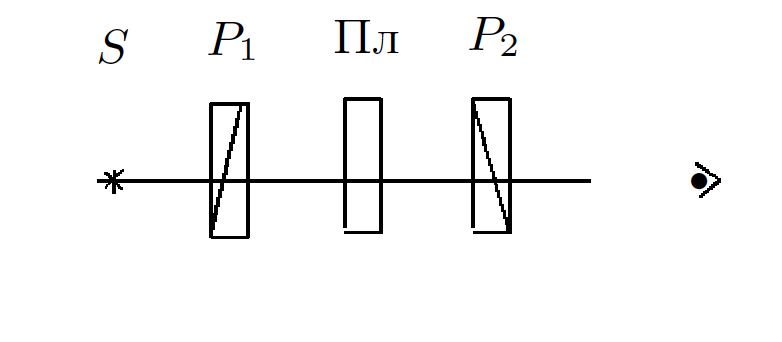
\includegraphics[width=\linewidth]{7}
	\caption{Разложение элептической поляризации на линейные компоненты}
	\label{ris 1}
\end{wrapfigure}
При помощи специальных приспособлений (поляризаторов), естественный свет может быть поляризован. Наиболее общим типом поляризации является \textit{эллиптическая поляризация}. В эллиптически поляризованной световой волне конец вектора \textbf{E} в данной точке пространства описывает некоторый эллипс. Линейно поляризованный свет можно рассматривать как частный случай эллиптически поляризованного света, когда эллипс поляризации вырождается в отрезок прямой линии; другим частным случаем является круговая
поляризация (эллипс поляризации является окружностью). \par
Для получения линейно поляризованного света применяются специальные оптические приспособления — поляризаторы. Направление колебаний электрического вектора в волне, прошедшей через поляризатор, называется
разрешенным направлением поляризатора. Всякий поляризатор может быть использован для исследования поляризованного света, т. е. в качестве анализатора. Интенсивность I линейно поляризованного света после прохождения через анализатор зависит от угла, образованного плоскостью колебаний с разрешенным направлением анализатора:
\begin{equation}
    I = I_0 \cos^2\alpha.  
\end{equation}
Соотношение (1) носит название \textit{закона Малюса}. \par
Отраженный от диэлектрика свет всегда частично поляризован. Степень поляризации света, отраженного от диэлектрической пластинки в воздух, зависит от показателя преломления диэлектрика $n$ и от угла падения $\varphi$. Как следует из формул Френеля, полная поляризация отраженного света достигается
при падении под \textit{углом Брюстера}, который определяется соотношением
\begin{equation}
    \tg \varphi = n.   
\end{equation}

В этом случае плоскость колебаний электрического вектора в отраженном свете перпендикулярна плоскости падения. Для увеличения степени поляризации преломлённого света используют стопу стеклянных пластинок, расположенных под углом Брюстера к падающему свету. \par

\textbf{Определение направления разрешенной плоскости колебаний поляроида.}\par
Луч света, прошедший поляроид и отразившийся от чёрного зеркала, имеет минимальную интенсивность при выполнении двух условий: во-первых, свет падает на отражающую поверхность под углом Брюстера, и во-вторых, в падающем пучке вектор E лежит в плоскости падения. \par
Вращая поляроид вокруг направления луча и чёрное зеркало вокруг оси, перпендикулярной лучу, методом последовательных приближений можно добиться минимальной яркости луча, отражённого от зеркала, и таким образом определить разрешённое направление поляроида. По углу поворота зеркала можно определить коэффициент преломления материала, из которого изготовлено зеркало \par

\textbf{Получение элептически поляризованного света и его анализ.}\par
Эллиптически поляризованный свет можно получить из линейно поляризованного с
помощью двоякопреломляющих кристаллических пластинок.

Двоякопреломляющая пластинка имеет два взаимно перпендикулярных главных направления, совпадающих с осями эллипсоида диэлектрической проницаемости. Волны, поляризованные вдоль главных направлений, распространяются в пластинке с разными скоростями, не изменяя характера своей поляризации. Обозначим показатели преломления для главных волн через $ n_x $ и $ n_y $, где $ x $ и $ y $ --- главные направления кристаллической пластинки. На входе пластинки $ E_x $ и $ E_y $ находятся в фазе, однако на выходе из-за разности скоростей между ними появляется разность хода $ d(n_x - n_y) $, при этом сдвиг фаз определяется соотношением:
\begin{equation}\label{}
    \Delta \phi =  \dfrac{2\pi}{m} = k d(n_x - n_y)
\end{equation}

Анализ эллиптически поляризованного света сводится к нахождению главных осей
эллипса поляризации и к определению направления вращения электрического вектора.

Главные оси эллипса поляризации определяются с помощью анализатора по максимуму и минимуму интенсивности проходящего света. Направление вращения электрического вектора может быть найдено с помощью пластинки в четверть длины волны, для которой известно, какая из главных волн, $ E_x $ или $ E_y $, имеет б\'{o}льшую скорость распространения.

\textbf{Пластинка чувствительного оттенка}\par
\begin{wrapfigure}{l}{0.35\linewidth}
	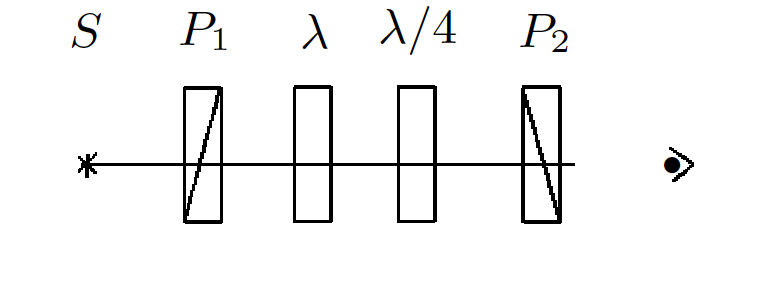
\includegraphics[width=\linewidth]{8}
	\caption{Пластинка чувствительного оттенка}
	\label{ris 3}
\end{wrapfigure}

Установить какому из двух главных направлений пластинки $\lambda/4$ соответствует большая скорость распространения света можно различными способами, например с помощью пластинки чувствительного оттенка.

Пластинка имеет форму стрелы (рис. 2), вдоль оси которой расположено главное направление, соответствующее большей скорости распространения.

Если пластинка чувствительного оттенка помещена между скрещенными поляроидами и главные направления пластинки не параллельны направлениям разрешённых колебаний поляроидов, то при освещении белым светом пластинка кажется окрашенной в лилово-красный цвет.

Если между скрещенными поляроидами поместить пластинку чувствительного оттенка и пластинку в $ \lambda/4 $ так, чтобы их главные
направления совпадали, то проходящий свет будет казаться зеленовато-голубым.
Если же главные направления, соответствующие большей скорости распространения, у пластинки чувствительного оттенка и у пластинки
в $ \lambda/4 $ окажутся перпендикулярными, то проходящий свет приобретёт
оранжево-желтую окраску.

Изменение цвета позволяет, таким образом, определить, какое из
главных направлений пластинки в $ \lambda/4 $ соответствует большей скорости
распространения.
\newpage
\textbf{Интерференция поляризованных лучей.}\par
\begin{wrapfigure}{r}{0.35\linewidth}
	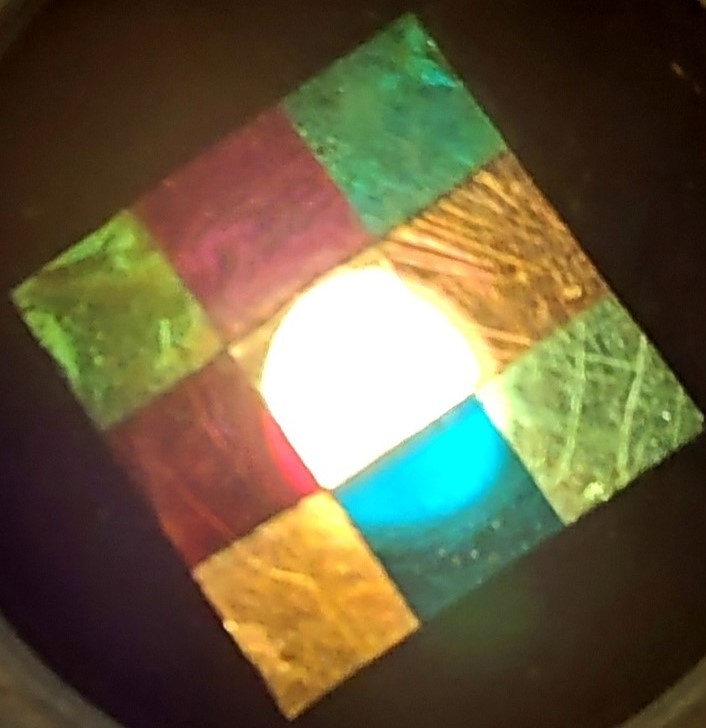
\includegraphics[width=\linewidth]{9}
	\caption{К объяснению интерференции поляризованных лучей}
	\label{ris 4}
\end{wrapfigure}

Тонкие двоякопреломляющие пластинки, помещённые между поляроидами, кажутся окрашенными. Эта окраска может быть истолкована как результат интерференции поляризованных лучей. На рис. 3 представлена схема для
случая скрещенных поляроидов.

Здесь $ p_{1}p'_{1} $ --- разрешённое направление колебаний поляризатора
(первого поляроида); $ x, y $ --- координатная система, связанная с главными направлениями двоякопреломляющей пластинки; $ p_{2}p'_{2} $ --- разрешённое направление колебаний анализатора (второго поляроида). Волны
$ E_x  $ и $ E_y $ на выходе из пластинки когерентны, но не могут интерферировать, так как $ E_x \perp  E_y $. Волны $ E_1 $ и $ E_2 $ на выходе второго поляроида
также являются когерентными и к тому же поляризованы в одной плоскости. Эти волны интерферируют между собой. Результат интерференции определяется зависящим от длины волны сдвигом фаз между $ E_1 $
и $ E_2 $. В результате интерференции поляризованных лучей пластинка, освещаемая белым светом, кажется окрашенной.


\section*{3.Ход работы}

\subsection*{3.1 Определение разрешенных направлений поляроидов}

Разместим на оптической скамье осветитель S, поляроид $P_{2}$ и черное зеркало так, чтобы плоскость падения была горизонтальна (рис.4). Свет, отраженный от зеркала, рассматриваем сбоку, расположив глаз таким образом, чтобы вблизи оси вращения зеркала можно было увидеть изображение диафрагмы осветителя

\begin{center}
    \includegraphics[scale = 0.5]{1.png}
    \captionof{figure}{Определение разрешенного направления поляроида}
\end{center}

Поворачивая поляроид вокруг направления луча, добьемся наименьшей яркости отраженного пятна. Оставим поляроид в этом положении и вращением зеркала вокруг вертикальной оси снова добьемся минимальной интенсивности отраженного луча.
Таким образом поляроид $P_{2}$ имеет горизонтальное разрешенное положение, соответствующее $\alpha = 306^{\circ}$

Разрешенное положение второго поляроида можно определить, скрестив поляроиды, т.е. поставив сначала поляроид $P_{2}$ с известной поляризацией, а затем $P_{1}$. Вращением второго поляроида добьемся минимальной яркости луча.
Тогда поляроид $P_{1}$ имеет вертикальное разрешенное положение, соответствующее $\alpha = 45^{\circ}$

\subsection*{3.2 Определение угла Брюстера для эбонита}

Поставим на скамью вместо черного зеркала эбонитовую пластину с круговой шкалой. Установив направление разрешенных колебаний поляроида $P_{2}$ горизонтально, найдем угол поворота эбонита $\varphi_{B}$, при котором интенсивность отраженного луча минимальна. Полученные измерения запишем в таблицу 1:

\begin{table}[H]
\begin{tabular}{|c|c|c|}
\hline
N & $\varphi_{B}$ & $\sigma_{\varphi_{B}}$          \\ \hline
1 & $57^{\circ}$  & \multirow{3}{*}{1} \\ \cline{1-2}
2 & $58^{\circ}$  &                    \\ \cline{1-2}
3 & $56^{\circ}$  &                    \\ \hline
\end{tabular}
\caption{Измерение угла Брюстера для эбонита}
\end{table}

Отсюда среднее значение $<\varphi_{B}> = (57 \pm 1)^{\circ}$

Добавив светофильтр, повторим измерения. Получим, что среднее значение $<\varphi_{B}>$ не меняется.

Рассчитаем показатель преломления эбонита по среднему значению угла Брюстера:

\begin{equation*}
    n = tg\varphi_{B} = 1,57\pm 0,59
\end{equation*} 

Здесь погрешность n мы считали по формуле:

\begin{equation*}
    \sigma_{n} = |\frac{1}{cos^2(\varphi_{B})}\cdot\sigma_{\varphi_{B}}|
\end{equation*} 

Полученное значение сходится с табличным ($n_{th} = 1,6 - 1,7$) в пределах погрешности

\subsection*{3.3 Исследование стопы}

Поставив стопу стеклянных пластинок вместо эбонитового зеркала, подберем для нее такое положение, при котором свет падает на стопу под углом Брюстера.

Осветим стопу неполяризованным светом и, рассматривая через поляроиды свет (рис.5), отраженный, а затем преломленный, определим ориентацию вектора Е. В итоге мы пришли к выводу, что отраженный свет обладает преимущественно вертикальной ориентацией, а преломленный - горизонтальной.

\begin{center}
    \includegraphics[scale = 0.5]{2.png}
    \captionof{figure}{Определение разрешенного направления поляроида}
\end{center}

\subsection*{3.4 Определение главных плоскостей двоякопреломляющих пластин}

Поставим кристаллическую пластинку между скрещенными поляроидами $P_{1}$ и $P_{2}$. Вращая пластинку вокруг направления луча и наблюдая за интенсивностью света, проходящего сквозь второй поляроид, определим, при каком условии главные направления пластинки совпадают с разрешенными направлениями поляроидов.

\begin{center}
    Пластина 1 \hspace{1cm} Пластина 2 \\
    $min: 102^{\circ}$ \hspace {1cm} $min: 280^{\circ}$ \\
     $max: 148^{\circ}$ \hspace {1cm} $max: 240^{\circ}$
\end{center}
Минимумы и максимумы интенсивности чередуются через $45^{\circ}$, главные плоскости пластин совпадают с разрешёнными направлениями поляроидов при максимальной интенсивности


\subsection*{3.5 Выделение пластин $\frac{\lambda}{4}$ и $\frac{\lambda}{2}$}

Добавим к схеме, изображенной на рисунке 6, зеленый фильтр, установим разрешенное направление поляроида горизонтально, а главные направления исследуемой пластинки - под углом $45^{\circ}$ к горизонтали.

\begin{center}
    \includegraphics[scale = 0.5]{3.png}
    \captionof{figure}{Определение главных направлений в пластинках}
\end{center}

С помощью второго поляроида установим, какую поляризацию имеет свет:

Пластинка 1 ($\frac{\lambda}{4}$):
интенсивность не менялась при повороте. Следовательно, мы имеем дело с круговой поляризацией, т.е. пластинка 1 - пластинка $\frac{\lambda}{4}$, создающая сдвиг фаз $\pi/2$ между колебаниями.

Пластинка 2 ($\frac{\lambda}{2}$):
интенсивность изображения менялась при повороте пластинки, т.е. линейная поляризация. Получается, что данная пластинка 2 - пластинка $\frac{\lambda}{2}$, не меняющая характер поляризации.

\subsection*{3.6 Определение направлений большей и меньшей скорости}

Поставим между скрещенными поляроидами пластинку чувствительного оттенка ($\lambda$ для зеленого света), имеющую вид стрелки. Световой вектор проходит с большей скоростью вдоль стрелки, с меньшей - перпендикулярно.

Убрав зеленый фильтр, поставим между скрещенными поляроидами пластинку $\lambda$. Глядя сквозь через второй поляроид на стрелку, мы увидим, что она окрасилась в пурпурный цвет (зеленый свет задерживается вторым поляроидом, а красная и синяя компоненты проходят).

Добавим к схеме пластинку $\frac{\lambda}{4}$ (рис.7), главные направления которой совпадают с главными направлениями пластины $\lambda$ и ориентированы под углом $45^{\circ}$ к разрешенным направлениям скрещенных поляроидов. При повороте рейтера со стрелкой на $180^{\circ}$ вокруг вертикальной оси цвет стрелки меняется от зелено-голубого до оранжево-желтого.

\begin{center}
    \includegraphics[scale = 0.5]{4.png}
    \captionof{figure}{Определение направлений большей и меньшей скорости}
\end{center}

Рассмотрим немного подробнее этот процесс:

Если "быстрые" оси обеих пластин совпадают, то систему пластин можно представить как одну пластинку $\frac{5\lambda}{4}$. Пусть длина зеленого света 500нм, тогда наша пластинка работает, как пластинка $\lambda$, для красного света с длиной 625 нм, т.е. из всего спектра она не пропускает только красный. Следовательно, стрелка окрашивается в сине-зеленый цвет.

Аналогично, если "быстрые" оси обеих пластин не совпадают, то система пластинок может быть рассмотрена как пластинка $\frac{3\lambda}{4}$. Получается, что она не пропускает сине-фиолетовый свет с длиной волны 375-423 нм. Тогда стрелка окрашивается в оранжево-желтый цвет.

\subsection*{3.7 Интерференция поляризованных лучей}

Расположим между скрещенными поляроидами мозаичную слюдяную пластинку, собранную из 4-х узких полосок слюды, лежащих по сторонам квадрата (в центральном квадрате слюды нет). Главные направления всех пластинок ориентированы параллельно сторонам квадрата.

Вращая пластинку, пронаблюдаем за изменениями в отдельном квадратике. У нас изменяется интенсивность. 

Не трогая пластинки, вращаем второй поляроид. Отличие в том, что теперь изменяется цвет пластинок также с периодичностью  $\pi/4$ (рис.8а и рис.8б):

\begin{figure}[H]
\begin{minipage}[h]{0.49\linewidth}
\center{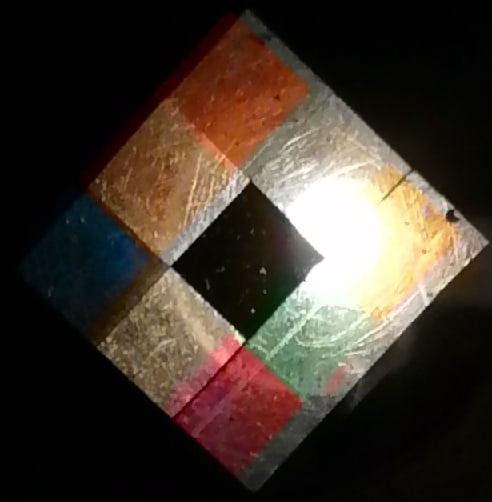
\includegraphics[width=0.6\linewidth]{5.jpg} \\ а)}
\end{minipage}
\hfill
\begin{minipage}[H]{0.49\linewidth}
\center{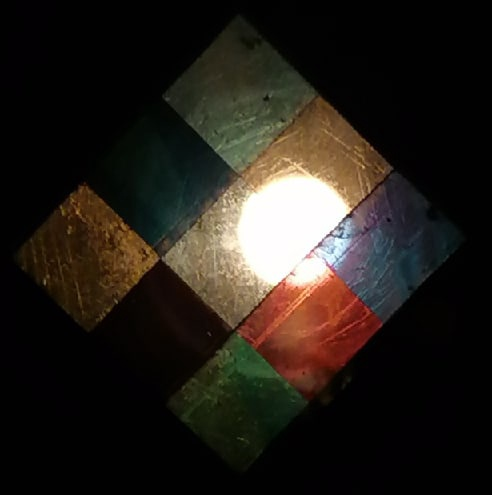
\includegraphics[width=0.6\linewidth]{6.jpg} \\ б)}
\end{minipage}
\caption{Интерференция поляризованных лучей}
\end{figure}


\section*{4. Вывод}

Мы ознакомились с методами получения и анализа поляризованного света. Провели несколько качественных экспериментов, с помощью которых узнали, как исследовать и создавать поляризованное излучение.
Определили разрешённые направления поляроидов.Экспериментально получили значение коэффициента преломления для эбонита $n=1,57\pm 0,59$, что в пределах погрешности сходится с теоретическими данными ($n=1,6-1,7$). Для двоякопреломляющих пластин определили главные направления, а так же тип пластинок --- $\lambda /4$ и $\lambda/2$. Также исследовали пластинку чувствительного оттенка, определили быструю и медленную оси и рассмотрели эффекты, происходящие при прохождении света через комбинацию пластинок. Получили эллиптически поляризованную волну, рассмотрели интерференцию поляризованных лучей в мозаичной слюдяной пластинке.


\end{document}

